\documentclass[]{llncs}

\usepackage[spanish]{babel}
\usepackage[dvipsnames]{xcolor}
\usepackage{mathtools}  
\usepackage{xfrac}  
\usepackage{graphicx}
\usepackage{subfigure}

%\newcommand{\Todo}[1]{\colorbox{BurntOrange}{#1}}
%\authorrunning{Matías Micheletto}
%\titlerunning{Agrar.io: Una aplicación multiplataforma para la gestión de tareas...}


\begin{document}

\title{Agrar.io: Una aplicación multiplataforma para la gestión de tareas agropecuarias}
\author{Dr. Matías Micheletto\orcidID{0000-0002-1891-3137}}
\institute{Sendevo Software, Bahía Blanca (8000), Buenos Aires \\ 
\email{matiasmicheletto@gmail.com}}

\maketitle

\begin{abstract}
En este trabajo se describen los detalles funcionales y técnicos de una aplicación multiplataforma orientada a la gestión integral de tareas agropecuarias. A partir de este desarrollo se destacan tres aportes principales: (1) la definición de un modelo ontológico para representar tareas agropecuarias, (2) la implementación de bases de datos distribuidas para compartir información punto a punto entre usuarios con escaso ancho de banda disponible y (3) la integración de estas propuestas en un único software multiplataforma, cuyas características de descentralización, flexibilidad y foco tanto en la privacidad como el soporte móvil offline, lo convierten en un producto que se diferencia respecto de otras alternativas dentro del mercado digital actual. Este desarrollo está pensado para brindar un conjunto de utilidades a un amplio espectro de usuarios pertenecientes al ámbito agropecuario, como productores, profesionales, asesores y/o contratistas.

\keywords{Ontologías \and Desarrollo web \and IPFS \and PWA \and Android.}
\end{abstract}

\section{Introducción}

Durante el transcurso de los últimos años, el advenimiento de la inteligencia artificial (AI, por sus siglas en inglés) está revolucionando el desarrollo de productos tecnológicos en múltiples ámbitos. En el contexto de la producción agropecuaria, una de las potenciales aplicaciones de la AI es la automatización de la toma de decisiones, la cual, en un sentido amplio, es un desafío que aún sigue sin resolverse \cite{ulitin2019,bao2022,schmitt2023}. Esta tarea requiere de un volumen de datos considerable, los cuales deben estar bien estructurados y organizados para garantizar la eficacia del modelo \cite{beleites2013,figueroa2012}. 

Por esta razón es que resulta fundamental contar con un formato de datos que permita modelar las tareas agropecuarias, el momento y el lugar en que se realizan, así como también los motivos por los cuales se ejecutan, como por ejemplo, las condiciones climáticas, valores de mercado, disponibilidad de insumos, etc. Si bien se han desarrollado distintos modelos ontológicos para formalizar conceptos en el dominio de las tareas agropecuarias \cite{abrahao2017,abrahao2018}, no se han validado estas propuestas mediante el desarrollo de aplicaciones de software. Uno de los aportes de este trabajo consiste en la propuesta de un formato para modelar y describir digitalmente las características de distintas tareas que se realizan en el contexto de la producción agropecuaria. 

Una vez contando con un formato adecuado y flexible para representar un conjunto diverso de eventos que ocurren en el contexto agroproductivo, sólo resta avanzar con el ingreso de datos, es decir la populación de una base de datos lo suficientemente extensa a partir de la cual sea posible extraer información útil y entrenar modelos de aprendizaje automático que asistan a la toma de decisiones. Para lograr este objetivo se evidencia la necesidad de contar con un gran número de usuarios, una tarea que implica ofrecer un producto atractivo a un mercado digital competitivo y en constante crecimiento, lo cual representa un desafío considerable. 

En la actualidad, las principales plataformas digitales con las que es posible registrar o documentar tareas agropecuarias, poseen algunas características que imponen cierta \textit{fricción} al usuario \cite{encuesta}, es decir, limitaciones que previenen a los usuarios de lograr ciertos objetivos o tareas con facilidad mediante el uso del sistema. La característica más recurrente es el requerimiento del registro o identificación del usuario, que atenta contra la privacidad del mismo, al tener que revelar algunos datos personales y configurar factores de autenticación. Otra limitación que se presenta en muchos sistemas, es el tiempo que se debe destinar al ingreso de datos, por ejemplo, de campos, lotes, maquinarias, animales, etc. antes de poder ejecutar cualquier acción, como generar órdenes de labor, ejecutar análisis con herramientas propias del sistema o compartir información con otros usuarios.

Con el objetivo de resolver, al menos en parte, las problemáticas expuestas anteriormente, se procedió con el diseño e implementación de un software multiplataforma que, operando con un sistema de archivos descentralizado, ofrece al usuario soporte offline prolongado, una base de datos para el registro y consulta de tareas agropecuarias, mecanismos de edición colaborativa de datos y múltiples herramientas de cálculo. Se presentan en este artículo, los requerimientos planteados, la arquitectura propuesta y los detalles más relevantes acerca del funcionamiento del sistema. 

El resto del trabajo se organiza de la siguiente manera: en la sección \ref{sec:modelo} se describe el modelo ontológico empleado para representar a las tareas agropecuarias, se proponen dos ejemplos ilustrativos y se discuten distintos casos de uso. En la sección \ref{sec:datos} se presenta el sistema de archivos que se propone y la relación entre las distintas bases de datos con las que funciona el sistema. En la sección \ref{sec:software} se discute la elección de la tecnología y se detallan las cuestiones técnicas involucradas en la implementación y el despliegue del software para múltiples plataformas. Finalmente, en la sección \ref{sec:conclusion} se concluye el trabajo, se enumeran los avances pendientes y posibles futuros pasos. 
\section{Modelo ontológico de tareas agropecuarias} \label{sec:modelo} 

Las tareas agropecuarias son variadas dado el amplio espectro de productos y subproductos que se generan en esta actividad y las numerosas técnicas que son empleadas en el ámbito. Ejemplos de tareas agropecuarias pueden ser la siembra de cultivos desde cereales u oleaginosas hasta especies arbóreas, el arreo de ganado para cambio de lotes durante el pastoreo, el encierre y ordeñe de animales en tambos, las tareas de fertilización o riego de cultivos, la recolección y transporte de huevos en granjas apícolas o la construcción y mantenimiento de infraestructuras como silos, molinos o galpones, por mencionar algunos casos particulares. 

En general podría decirse que una actividad agropecuaria puede ser descripta indicando el nombre de la tarea, el lugar y el momento en que se realiza, la o las personas encargadas de llevarla a cabo, los detalles de cómo se realizará esta tarea y los motivos por los que se ejecuta. Es decir, la descripción se realiza respondiendo a una serie de pronombres interrogativos que, en el contexto del periodismo y criminalística, se los suele conocer como las ``5W y 1H'', los cuales son: qué, dónde, cuándo, quién/quiénes, cómo y por qué.

Teniendo en cuenta este esquema, se propone un modelo de tarea que se compone de secciones donde cada una contiene una lista de ítems clasificados según la siguientes categorías:

\begin{itemize}
    \item \textbf{Actividad (qué):} este ítem permite entender el contexto de la tarea. Las actividades pueden organizarse de forma jerárquica permitiendo establecer una taxonomía, por ejemplo ``siembra directa'' y ``siembra convencional'' son subtipos de ``siembra'' y que junto con ``pulverización'' son a la vez subtipos de ``labores de producción de cultivos''.
    \item \textbf{Ubicación (dónde):} dentro de esta sección es posible indicar el espacio geográfico en el cual se realizará la tarea. Existen, en el contexto de este sistema, tres tipos de ubicaciones: marcadores (un sitio puntual), líneas (trayectoria compuesta por la unión de múltiples puntos) y  polígonos (la superficie contenida en un conjunto de al menos tres puntos). Los marcadores permiten ubicar actividades puntuales, como el emplazamiento de un galpón o un molino. Las líneas pueden emplearse para describir caminos, alambrados o silos de pastura picada. Finalmente, los polígonos son apropiados para delimitar e identificar parcelas, lotes o campos.
    \item \textbf{Fechas (cuándo):} la fecha indica el momento o periodo de tiempo pasado o futuro en que fue realizada o se realizará la tarea en cuestión.
    \item \textbf{Personas (quién/quiénes):} este ítem hace referencia a la o las personas físicas o jurídicas encargadas de realizar la tarea, o que de manera indirecta guardan alguna relación con esta tarea.
    \item \textbf{Razones (por qué):} se introduce este ítem para describir los motivos por los que se realiza cierta tarea, por ejemplo, condiciones climáticas o de mercado, oportunidad, entre otras.
    \item \textbf{Parámetros (cómo):} esta sección contiene variables y parámetros con sus respectivos valores y unidades de medida y demás detalles descriptivos que permitan conocer la configuración utilizada en las herramientas o la forma en que debe ejecutarse la tarea.
\end{itemize}

\subsection{Ejemplos}
A continuación se muestran dos ejemplos de tareas agropecuarias que son descriptas empleando el modelo propuesto. Se proponen dos tareas de características diferentes, como lo son las labores con maquinaria en producción de cultivos, en el ejemplo, pulverización de un lote y por otro lado, la construcción de infraestructura para ganado, en este caso, un alambrado tradicional.

\subsubsection{Ejemplo 1: Barbecho químico sobre lote.} Este ejemplo ilustra los datos registrados en el caso de la realización de una pulverización con agroquímicos como tarea de preparación (barbecho) de un lote de 60 has. por parte de un contratista hipotético (Contratista X). En el campo de fecha se establece un período de aplicación recomendado dentro del cual deben buscarse las condiciones climáticas apropiadas. Por último, en la descripción se especifican los parámetros operativos como volumen de pulverización y presión de trabajo del equipo y los insumos a aplicar, junto con el correspondiente porcentaje de dilución.
\begin{itemize}
    \item \textbf{Actividad (qué):} Cultivos $\rightarrow$ Pulverización.
    \item \textbf{Ubicación (dónde):} Lote IV (polígono georeferenciado de 60 has). 
    \item \textbf{Fechas (cuándo):} Entre el 23/02/2023 y el 28/02/2023.
    \item \textbf{Personas (quién/quiénes):} Contratista X. 
    \item \textbf{Razones (por qué):} Barbecho químico previo a siembra de avena. 
    \item \textbf{Parámetros (cómo):} 
    
    \begin{center}
        \begin{tabular}{ |l|r|c| } 
            \hline
            \textbf{Parámetro} & \textbf{Valor} & \textbf{Unidad} \\ 
            \hline
            Capacidad de tanque & 3000 & l \\ 
            Volumen de pulverización & 50 & l/ha \\ 
            Presión de trabajo & 2 & bar \\ 
            Glifosato & 3 & l/ha \\ 
            2,4D & 0.8 & l/ha \\ 
            Coadyuvante & 60 & ml/100 l \\ 
            \hline
        \end{tabular}
        \quad
        \begin{tabular}{ |l|r|c| } 
            \hline
            \textbf{Insumo} & \textbf{Total} & \textbf{Unidad} \\ 
            \hline
            Agua & 3000 & l \\ 
            Glifosato & 180 & l \\ 
            2,4D & 48 & l \\ 
            Coadyuvante & 1.8 & l \\ 
            \hline
        \end{tabular}
    \end{center}
\end{itemize}

\subsubsection{Ejemplo 2: Construcción de un alambrado.} La tarea de este ejemplo describe la construcción de un alambrado tradicional a lo largo de un emplazamiento especificado mediante coordenadas gps. Similarmente al caso anterior se asigna la tarea a un contratista hipotético y dentro de los parámetros se especifica el tipo de alambrado y los insumos totales requeridos.

\begin{itemize}
    \item \textbf{Actividad (qué):} Infraestructura $\rightarrow$ Construcción.
    \item \textbf{Ubicación (dónde):} Alambrado (línea recta georeferenciada de 350 m). 
    \item \textbf{Fechas (cuándo):} 05/03/2023.
    \item \textbf{Personas (quién/quiénes):} Alambrador X. 
    \item \textbf{Razones (por qué):} Subdivisión de lote. 
    \item \textbf{Parámetros (cómo):} 

    \begin{center}
        \begin{tabular}{ |l|r|c| } 
            \hline
            \textbf{Parámetro} & \textbf{Valor} & \textbf{Unidad} \\ 
            \hline
            Cant. hilos & 7 & hilos \\  
            Medida claro & 12 & m \\ 
            Varillas/claro & 7 & u \\   
            \hline
        \end{tabular}
        \begin{tabular}{ |l|r|c| } 
            \hline
            \textbf{Insumo} & \textbf{Total} & \textbf{Unidad} \\ 
            \hline
            Alambre ovalado $\sfrac{17}{15}$ & 2500 & m \\ 
            Alambre dulce & 50 & m \\ 
            Varilla ceb. $\sfrac{11}{2}\cdot\sfrac{11}{2}\cdot1.2$ m & 210 & u \\ 
            Poste quebracho 2.5 m & 30 & u \\ 
            Torniquete golondrina & 14 & u \\ 
            \hline
        \end{tabular}
    \end{center}
\end{itemize}

Ambos ejemplos pueden modelar tanto un presupuesto elaborado por el contratista como una orden de trabajo generada por un productor o profesional, dependiendo del contexto, pero explican una misma tarea que se realizó o que se pretendía ejecutar en algún momento. Si bien los dos casos ilustran actividades diferentes, al estar enmarcadas en un mismo formato, es posible recompilar información útil, extraer patrones o simplemente realizar consultas sobre una misma base de datos en la que fueron registradas estas tareas, como se muestra más adelante, en la sección \ref{sec:db_query}.

En la sección \ref{sec:software} se detallan las cuestiones técnicas relacionadas con la definición del formato para la representación de cada sección del modelo de tareas y con el fin de ilustrar el potencial del modelo, se ejemplifican distintos casos de uso por medio de la generación de consultas que se pueden realizar a la base de datos para extraer información útil.
\section{Almacenamiento de datos} \label{sec:datos}

En términos generales, la funcionalidad más relevante de la aplicación es su capacidad para registrar y recuperar datos de forma eficiente y combinar datos de múltiples fuentes para obtener información útil. En este sentido se propone un sistema de archivos compuesto por cuatro tipos principales de bases de datos, lo que, en el contexto de la ingeniería de software, se conoce como ``persistencia políglota''. El primer tipo corresponde a las bases de datos privadas del usuario, que permiten registrar: 1) contactos de personas o empresas, 2) ubicaciones como marcadores, lotes o caminos y 3) tareas agropecuarias. El segundo tipo corresponde a las bases de datos colaborativas, que consisten en colecciones de datos que se pueden generar, modificar y distribuir libremente entre usuarios y que pueden emplearse para distintos propósitos dentro del contexto del sistema, como agilizar procesos de cálculo, autocompletar formularios o simplemente consultar información. El tercer tipo de base de dato dispone de herramientas de consulta, es decir, esquemas de filtrado y búsqueda que se pueden ejecutar sobre la base de datos de tareas agropecuarias de manera que sea posible extraer información útil para el usuario. Finalmente, el cuarto tipo de base de dato contiene herramientas de cálculo, donde cada una está compuesta por un formulario para el ingreso de parámetros de entrada y una librería de fórmulas matemáticas o procedimientos lógicos para generar resultados o parámetros de salida en formato compatible con el campo correspondiente a la sección de parámetros de las tareas.

Por cuestiones de seguridad y de complejidad de implementación, el diseño actual del software no admite la edición colaborativa de las bases de datos de las herramientas de consulta y cálculo, pero es una característica que es completamente factible de incorporar al sistema para convertirlo en una plataforma que admita el intercambio de este tipo de información y de esta manera, generar un potencial mercado de conocimiento \cite{kafentzis2004}, particularmente aplicado a los negocios agropecuarios. 

A continuación se describen las características de cada tipo de base de datos, el propósito de cada una, los distintos casos de uso y potenciales aplicaciones. Finalmente se ilustran los componentes y las relaciones entre cada uno en el esquema de la Figura \ref{fig:ontologia}.

\subsection{Bases de datos privadas} \label{sec:db_priv}
% lotes, contactos -> documentos (tareas)
La aplicación cuenta con tres bases de datos locales para almacenar información privada del usuario: contactos, ubicaciones y tareas. No se emplearon sistemas relacionales para implementar estas bases de datos, para mantener flexibilidad en cuanto al formato de los datos durante el desarrollo, aunque esto se logra al costo de un menor rendimiento en materia de velocidad para búsqueda y consulta. Este esquema resulta conveniente para el caso de prototipos como lo es el desarrollo que se propone en este trabajo, pero no es la alternativa más apropiada para lograr que el producto escale manteniendo un buen rendimiento computacional en el largo plazo.

\subsection{Bases de datos colaborativas} \label{sec:ipfs}
% info gral (productos, insumos, parámetros, cultivos, etc)
El proceso de carga de datos a un sistema mediante \textit{data entry} es costoso y no garantiza la completa disponibilidad de la información que el usuario muchas veces desea manejar, por lo que en este desarrollo se optó por el empleo de una alternativa conocida como \textit{crowdsourcing} o \textit{crowd sensing}, la cual consiste en permitir la recolección de datos colaborativa y voluntaria por parte de los mismos usuarios \cite{boubiche2019}.

A modo de servicio independiente dentro de la aplicación que se detalla en este trabajo, se propone el uso de un sistema de archivos distribuido para editar de forma colaborativa y compartir datos genéricos que resulten útiles dentro de la aplicación. A continuación se listan ejemplos de bases de datos que actualmente se incluyeron en la primera versión del software y se enumeran los posibles casos de uso de cada una.

\begin{itemize}
    \item \textbf{Actividades agropecuarias}: esta base de datos sugiere una categorización u organización jerárquica de actividades. Se emplea para darle contexto a una tarea registrada por el usuario.
    \item \textbf{Propiedades de cultivos}: como peso de mil semillas, peso por metro cúbico y ángulo de reposo de granos. Esta información es útil para realizar cálculos de siembra y almacenaje de granos. También es posible incluir otras propiedades como requerimientos hídricos, o recomendaciones de producción.
    \item \textbf{Propiedades de agroquímicos}: marcas, dosis recomendadas, forma de acción, precauciones de uso, etc. Permite consultar información y autocompletar campos con nombres extensos de productos para agilizar la generación de recetas, órdenes de labor o registrar inventarios.
    \item \textbf{Requerimientos hídricos de ganado}: valores de requerimientos hídricos diarios de distintas especies y categorías de animales, lo que permite estimar aguadas como tanques y bebederos o calcular molinos y bombas de extracción de agua de pozo según cantidad de cabezas.
    \item \textbf{Modelos de molinos}: propiedades de los modelos de molinos más utilizados, entre las que aparecen diámetro de rueda, altura, diámetro de cañerías, cilindros y varillas y los resultantes valores de caudal de agua. 
    \item \textbf{Insumos para alambrados}: tipos de alambre, varillas, postes y torniquetes empleado en el cálculo de insumos para la construcción de alambrados tradicionales.
\end{itemize}    

Se espera que en el futuro los usuarios puedan consultar la disponibilidad de las distintas bases de datos según sean requeridas y que sea posible editar libremente el contenido a partir de la creación de réplicas, ya que para evitar conflicto de formatos y tipos, las bases de datos son de sólo lectura. Por este motivo, para descargar una base de datos del sistema distribuido, un usuario debe conocer el identificador de contenido (CID, por sus siglas en inglés) de la base de datos correspondiente, que se calcula a partir de una función hash. Se detallan las cuestiones técnicas referidas a la implementación de este sistema de archivos distribuido en la sección \ref{sec:comunicacion}.

\subsection{Herramientas de consulta} \label{sec:db_query}
% extracción de información de la base de datos de documentos
De forma general, se podría decir que crear una consulta para una base de datos consiste en redactar una serie de condiciones que debe cumplir cada uno de los datos del conjunto que se desea recuperar. En el caso del modelo de datos que se emplea para la base de datos de tareas agropecuarias, es posible desarrollar una gran variedad de consultas para extraer información útil. En la siguiente lista se enumeran algunos ejemplos de consultas con distinto nivel de complejidad en su lógica, que es posible aplicar para recuperar información de la base de datos de tareas.

\begin{itemize}
    \item Listar todas las labores realizadas en un mismo lote a lo largo de la última campaña, o de cualquier periodo de tiempo especificado.
    \item Obtener la suma de precipitaciones acumulada durante el año actual y comparar el valor con la media histórica anual.
    \item Calcular la cantidad de insumos o materiales totales utilizados durante cierto periodo de tiempo o en cierta ubicación.
    \item Calcular la superficie total dada a trabajar a un mismo contratista durante el último año o la cantidad de kilómetros total contratada a cierto transportista, ya sea de cereales, ganado o cualquier producto.
\end{itemize}

Estas consultas se desprenden a partir de distintos casos de usos que algunas plataformas de gestión agrícola resuelven de forma nativa. De manera similar a lo que ocurre con las bases de datos, el hecho de que exista la posibilidad de que los mismos usuarios puedan editar y compartir sus propias herramientas de consulta, permitiría generar un espacio virtual para la creación de conocimiento de gran valor para el sector agropecuario.

\subsection{Herramientas de cálculo} \label{sec:calculos}
% modelos de calculo: formularios + ecuaciones = parametros
En el contexto de la plataforma que se presenta, las herramientas de cálculo combinadas con las bases de datos permiten, en cierta manera, modelar conocimiento y compartirlo entre usuarios. El modelo de cálculo que se emplea en esta plataforma consiste en dos elementos principales: un formulario para el ingreso de variables y una librería de fórmulas o algoritmos para el cálculo de los resultados, siendo estos últimos expresados en el formato de parámetros, el cual fue formalizado en la sección \ref{sec:modelo}. Este modelo fue pensado para cubrir un amplio conjunto de herramientas de cálculo y que pueda ser utilizado por los mismos usuarios para desarrollar sus propias herramientas.

Debido a que el software propuesto aún no dispone de interfaces para la creación, distribución, búsqueda y descarga de herramientas de cálculo por parte de los usuarios, la aplicación se distribuye con una serie de herramientas de cálculo precargadas y que se enumeran en la siguiente lista junto con una breve descripción de cada una.

\begin{itemize}
    \item \textbf{Parámetros de pulverización}. Permite determinar los parámetros operativos de pulverizadoras de arrastre. Las ecuaciones fueron extraídas del trabajo presentado en \cite{criollo}.
    \item \textbf{Parámetros de siembra}. Similar al caso anterior pero aplicado a todo lo relacionado con la siembra de granos gruesos, finos y tanto convencional como directa. Basado en el trabajo presentado en \cite{campero}.
    \item \textbf{Insumos de pulverización}. Esta calculadora permite determinar la cantidad de insumos totales dados los parámetros de aplicación y la superficie a pulverizar. Estas ecuaciones también fueron tomadas del trabajo presentado en \cite{criollo}.
    \item \textbf{Merma por humedad de granos}. Permite calcular la pérdida de peso de granos durante el secado. Esta calculadora emplea la base de datos de cultivos que contiene valores de humedad aceptable para cada variedad.
    \item \textbf{Almacenaje de granos}. Esta herramienta permite determinar el peso almacenado en silos tipo torre de base plana o cónica y galpones a partir de las dimensiones. Esta calculadora emplea la base de datos de cultivos para obtener los valores de ángulo de reposo de los distintos granos.
    \item \textbf{Dimensionamiento de aguadas}. Esta calculadora permite estimar volúmenes de aguadas y tamaño de molinos requeridos según la cantidad de cabezas de ganado. Para agilizar los cálculos, se puede emplear una base de datos de requerimientos hídricos de las distintas especies y categorías de animales.
\end{itemize}

\begin{figure}[t]
    \centering
    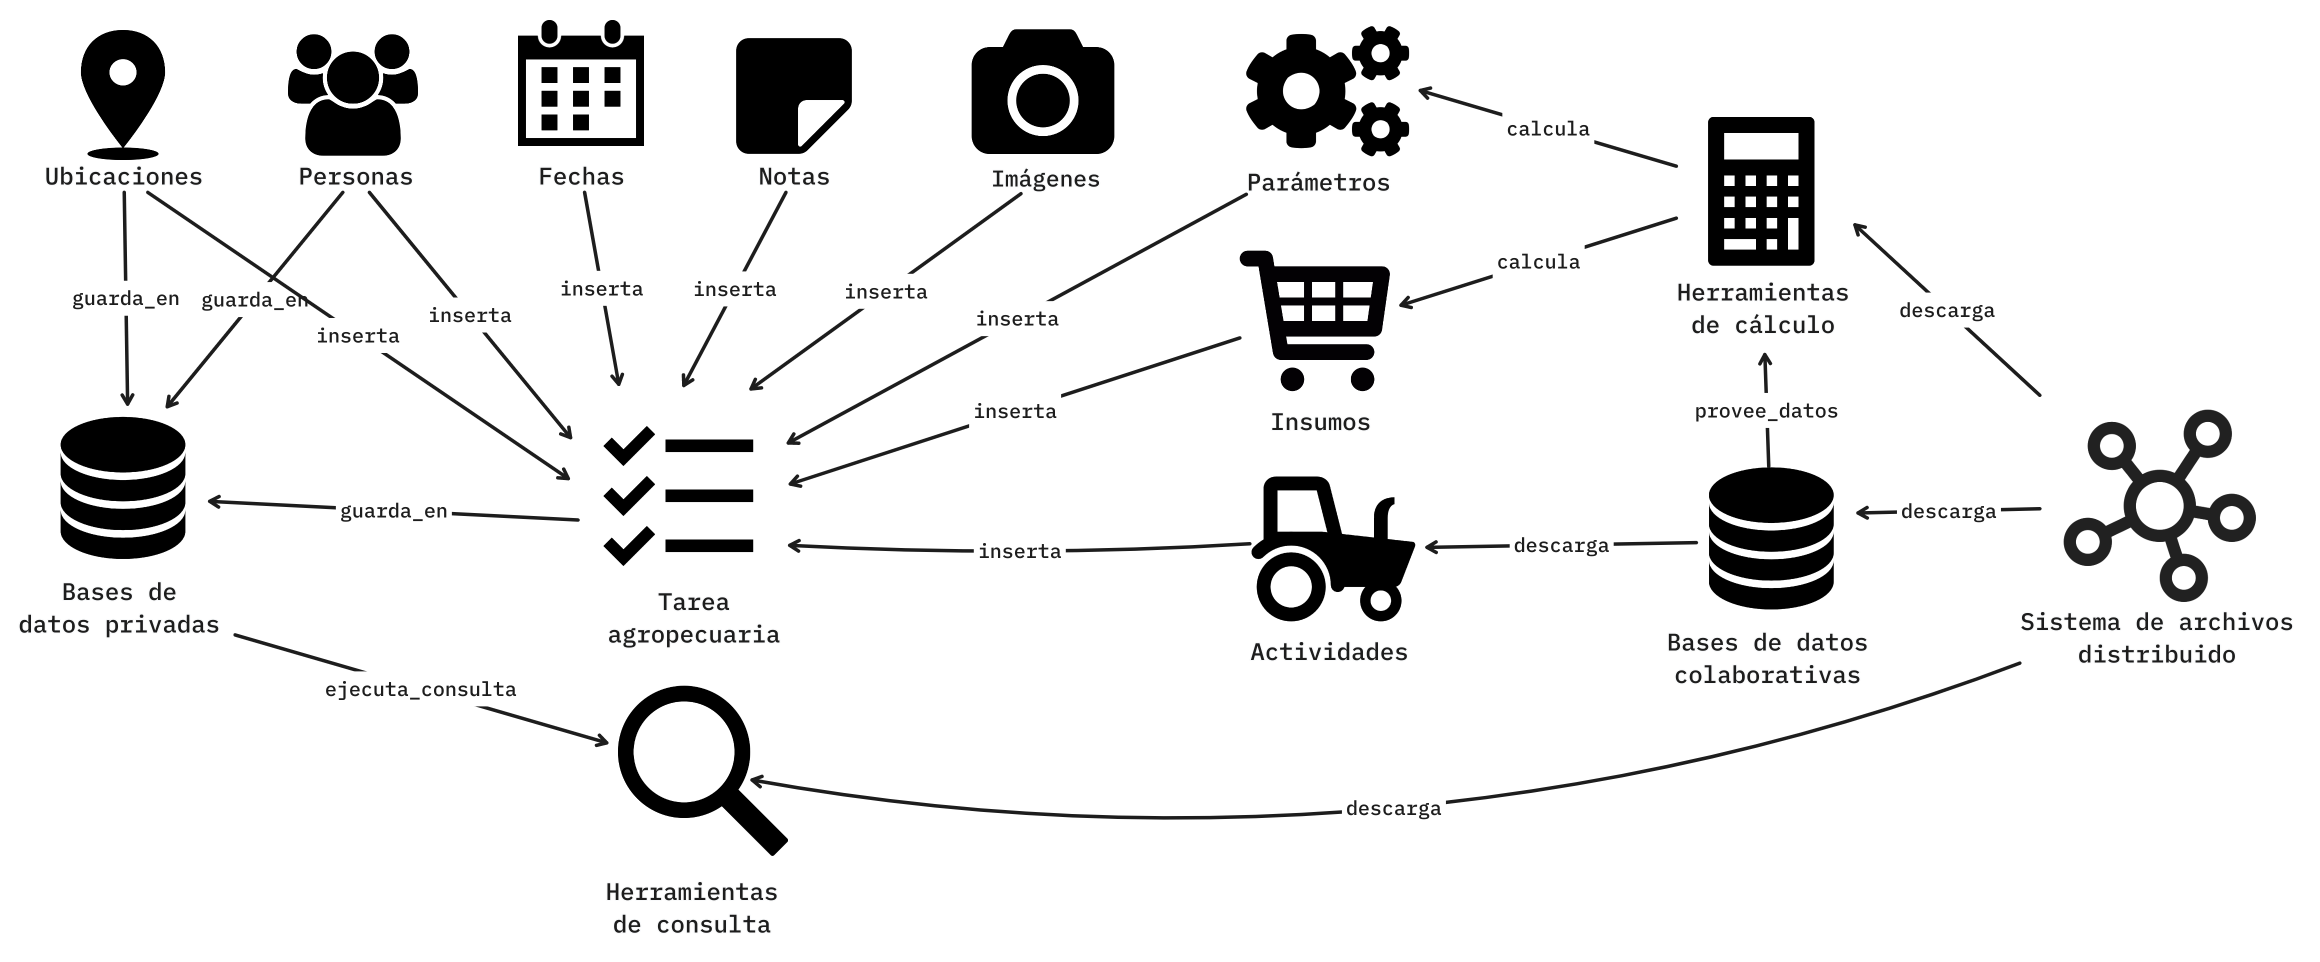
\includegraphics[width=\textwidth]{imagenes/ontologia2_lowres.png}
    \caption{Componentes del sistema y relaciones.} \label{fig:ontologia}
\end{figure}


\section{Implementación} \label{sec:software}

Con el objetivo de distribuir el software para múltiples plataformas a partir de la misma base de código, se emplearon lenguajes de programación web, principalmente, HTML5, JavaScript, CSS y las extensiones de estos lenguajes: TypeScript, Sass y JSX. La tecnología web tiene la ventaja de generar un software encapsulado en documentos que son compatibles con un amplio espectro de dispositivos, dado que se ejecutan en el contexto de navegadores web como Google Chrome o Mozilla Firefox, los cuales pueden ser instalados en computadoras personales, teléfonos inteligentes, \textit{Smart TVs}, \textit{Smart watches}, entre muchos otros. Por otro lado, el inconveniente que se presenta desde el punto de vista tanto comercial como de seguridad, es que el código fuente queda disponible y es accesible por parte del usuario para ser manipulado, copiado o alterado \cite{jazayeri}. En esta sección se enumeran las tecnologías utilizadas para el desarrollo de la propuesta y se describen brevemente las principales consideraciones que fueron tenidas en cuenta durante la construcción del sistema.

\subsection{Entorno de desarrollo}
El proyecto se implementó empleando a Vite\footnote{https://vitejs.dev/} como herramienta de gestión del código fuente y dependencias. Este software provee una serie de utilidades que agilizan el desarrollo del proyecto, particularmente del \textit{``front-end''}, como por ejemplo un servidor local con \textit{``hot reloading''}, un empaquetador o \textit{``bundler''} y una serie de comandos para el despliegue y testeo de la aplicación para distintos entornos.

El proyecto consta de múltiples puntos de entrada que apuntan a distintos objetivos de compilación: 1) una versión web \textit{on-line}, 2) una versión de escritorio y 3) una versión móvil. Las versiones de escritorio y móvil emplean componentes nativos de los distintos sistemas operativos, y que se acceden a través de \textit{``APIs''} tal como se describe en la sección \ref{sec:nativo}. La versión \textit{on-line} dispone de acceso limitado a ciertas herramientas y funcionalidades, para proteger recursos como \textit{API tokens} o código fuente de lógicas de negocio sensibles o que no se desea que sean accesibles por parte del usuario. Para lograr múltiples puntos de entrada en un proyecto \textit{``monorepo''}, se editaron los comandos de compilación del gestor de paquetes \textit{NPM}\footnote{https://www.npmjs.com/} indicando un archivo de configuración de Vite para cada objetivo. Este esquema permite reutilizar lógica y componentes entre las distintas versiones y mantener cada una con mínimo esfuerzo.

\subsection{Componentes nativos} \label{sec:nativo}
El esquema de desarrollo híbrido permite generar software ejecutable a partir de una aplicación web, lo que posibilita el funcionamiento de la misma de forma \textit{off-line}, de manera similar al esquema de aplicación web progresiva (PWA, por sus siglas en inglés), con la ventaja de que es posible acceder a utilidades nativas por medio de \textit{plugins} o APIs. Para lograr esto en plataformas móviles se utilizó CapacitorJS\footnote{https://capacitorjs.com/} y en el caso de sistemas operativos de escritorio como Windows o Linux, ElectronJS\footnote{https://www.electronjs.org/es/}. La versión compatible con sistemas operativos Android se puede descargar desde la tienda de aplicaciones Google Play\footnote{https://play.google.com/store/apps/details?id=com.sendevo.agrario}.

\subsection{Almacenamiento local}
Para el almacenamiento persistente de datos se emplean distintas tecnologías dependiendo del objetivo de compilación. En todos los casos se emplean representación de datos por pares clave-valor (KVP, por sus siglas en inglés).

La versiones \textit{on-line} y PWA emplean \textit{``localStorage''}, que consiste en un espacio para el almacenamiento persistente de datos mediante KVP. Este sistema está limitado a un espacio de 5 Mb, aunque puede variar dependiendo del navegador web. Para extender el almacenamiento, se incluye opcionalmente una conexión a una base de datos remota basada en el servicio de Google Firebase\footnote{https://firebase.google.com/}, que actúa como backup o sistema de sincronización de los datos de usuario entre varios dispositivos.

En el caso de las versiones nativas, se hace uso de los \textit{plugins} provistos por los distintos \textit{frameworks}, como \textit{Capacitor Storage} o \textit{FileReader}, en el caso de ElectronJS. 

\subsection{Almacenamiento distribuido} \label{sec:comunicacion}
La posibilidad de compartir información entre distintos usuarios siempre ha sido una utilidad muy requerida en la gran mayoría de los productos de software y no es diferente en el caso de las herramientas digitales para el agro \cite{davis1989,venkatesh2003,briggerman2010,michels2020}. 

El desafío que se presenta en este caso es la falta de conectividad permanente, por lo que se debe recurrir a enlaces punto a punto. Una manera para lograr este objetivo es el uso de la conectividad Bluetooth, sin embargo existen algunas limitaciones de practicidad que hacen que esta tecnología no sea muy aplicada para este propósito.

En el caso de la propuesta que se presenta en este trabajo se optó por mecanismos de comunicación empleados por aplicaciones descentralizadas. Una tecnología que resuelve la problemática de compartir información sin la participación de un intermediario es el Sistema de Archivos Interplanetario (IPFS, por sus siglas en inglés) \cite{tschorsch2022}. Para implementar el protocolo mediante tecnología web se hizo uso de la librería JS-IPFS\footnote{https://js.ipfs.tech/}, que emplea WebRTC\footnote{https://webrtc.org/} como medio de comunicación entre navegadores, permitiendo ejecutar un nodo en el contexto del navegador web. 

Existen distintas consideraciones que deben tenerse en cuenta al momento de desarrollar y utilizar sistemas de almacenamiento distribuidos, ya que implica un cambio de paradigma en lo que respecta a los aspectos que garantizan la persistencia y disponibilidad de los datos \cite{guidi2021,shen2019}. 

Si bien existen soluciones desarrolladas sobre IPFS que resuelven la implementación completa para bases de datos distribuidas, como OrbitDB\footnote{https://orbitdb.org/} o GunJS\footnote{https://gun.eco/}, para una primera versión de la propuesta presentada en este trabajo y dado que no se requieren mecanismos avanzados de sincronización de datos entre pares, se optó por el desarrollo de métodos \textit{ad-hoc}, para reducir dependencias innecesarias. Entonces, para resolver el problema de la edición colaborativa de datos que se describió en la sección \ref{sec:datos}, se ejecuta un nodo local IPFS, que en conjunto con los mecanismos de almacenamiento local, permiten acceder y compartir datos entre pares. Si bien la versión actual de la propuesta no posee esta caraterística, es posible ejecutar el nodo IPFS en segundo plano mediante una API nativa, como se presentó en \cite{cristea2020}. 

\subsection{Interfaz gráfica}
La interfaz gráfica de usuario (GUI, por sus siglas en inglés) se implementó con la ayuda de React y MUI\footnote{https://react.dev/, https://mui.com/}. Estas herramientas de código abierto proveen una lista de componentes de propósito general listos para usar, como botones, menúes, formularios, entre otros. Además se incluyó una lista de íconos predefinidos\footnote{https://react-icons.github.io/react-icons}, reduciendo el costo de diseño gráfico. 

\begin{figure}[ht]
    \hfill
    \subfigure[Edición de tarea]{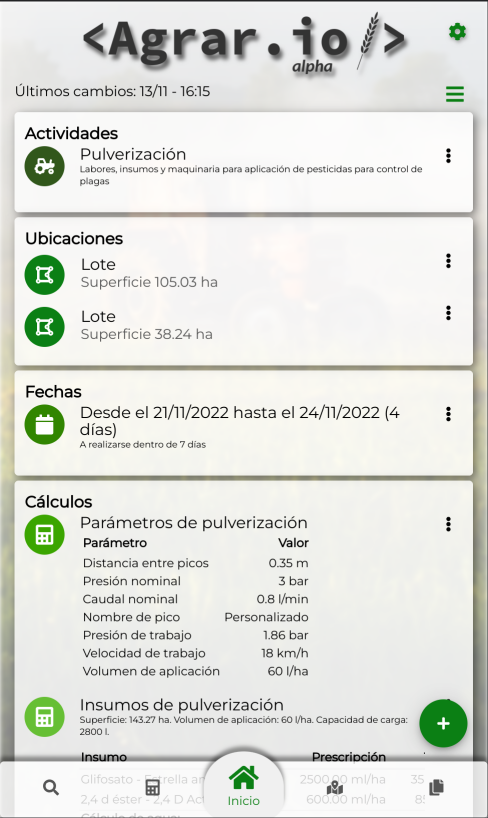
\includegraphics[width=0.3\textwidth]{imagenes/screenshot-0-lowres.png}}
    \hfill
    \subfigure[Edición de ubicaciones]{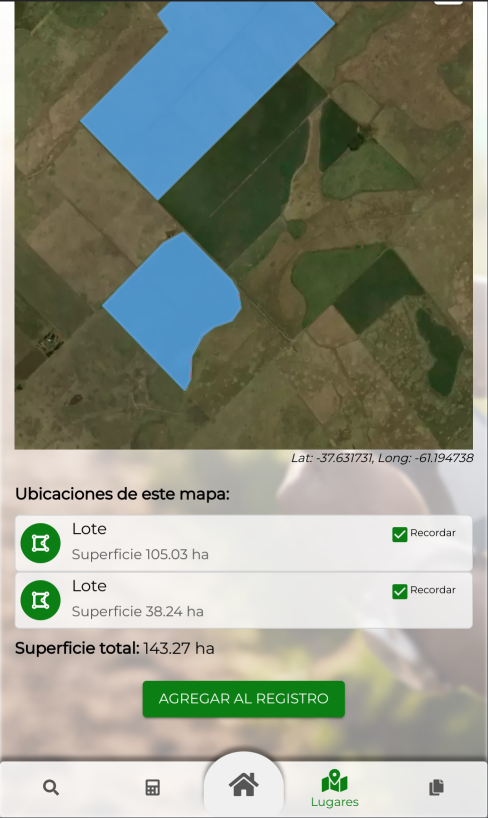
\includegraphics[width=0.3\textwidth]{imagenes/screenshot-5-lowres.png}}
    \hfill
    \subfigure[Cálculo de insumos]{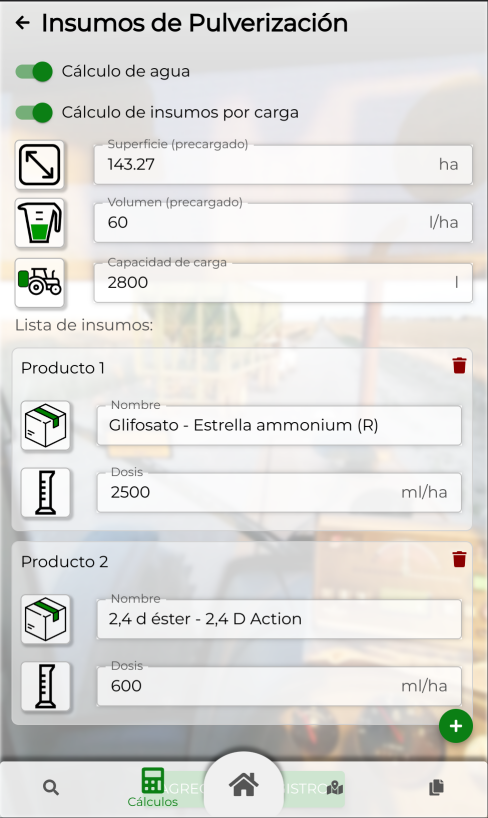
\includegraphics[width=0.3\textwidth]{imagenes/screenshot-6-lowres.png}}
    \hfill
    \caption{Capturas de pantalla de la aplicación} \label{fig:capturas}
\end{figure}

La traducción o cambio de idioma del contenido de las vistas se realiza con la ayuda del \textit{framework} de internacionalización \textit{i18next}\footnote{https://www.i18next.com/}, para el cual fueron definidos diccionarios en formato ``json'' con las traducciones de todos los términos que aparecen en la GUI. Actualmente sólo se cuenta con los idiomas español e inglés americano.

La Figura \ref{fig:capturas} muestra algunas capturas de pantalla de la aplicación móvil donde se puede observar las ventanas de edición documentos y de polígonos para lotes y a la derecha, una vista de cálculo de parámetros, particularmente de insumos de pulverización. Cada uno de estos menús posee un botón para insertar la información generada en el documento de tarea que se encuentra en edición. 


\subsection{Mapas}
Para permitir al usuario especificar ubicaciones georeferenciadas se incorpora una herramienta que facilita el dibujado de geometrías de manera gráfica sobre imágenes satelitales. De esta forma es posible ubicar marcadores, definir líneas o polígonos para indicar lotes o parcelas. Esta utilidad se implementó con la librería React-Map-GL, que emplea un servicio de MapBox\footnote{https://github.com/visgl/react-map-gl, https://www.mapbox.com/} para acceder a imágenes satelitales actualizadas. Este es un servicio gratuito siempre y cuando la cantidad de solicitudes de renderizado de mapas sea menor a una cota máxima. El formato que se utiliza para registrar las geometrías definidas por el usuario es GeoJSON\cite{geojson}, por razones de compatibilidad con el funcionamiento de MapBox y los métodos de conversión desde formatos KML o GPX, lo que facilita importar geometrías desde otras plataformas. Para los cálculos geoespaciales tales como distancias, superficies o determinación de centroides, se utilizó la librería TurfJS\footnote{https://turfjs.org/}.

\subsection{Clima y registro de variables}
La implementación actual de este software aún no cuenta con conexión a una interfaz de aplicación (API, por sus siglas en inglés) para obtener datos climáticos, pero se dispone de un formulario para el registro manual de variables definidas por el usuario y que se almacenan como parámetros, dentro de la base de datos de tareas. Esto permite realizar tareas de monitoreo o adquisición manual de datos.

Para complementar otros detalles que se quieran adicionar al registro de tareas, se dispone de un formulario para la redacción de notas de texto y también un espacio para adjuntar imágenes que se pueden cargar desde la galería de fotos del usuario o directamente capturar con la cámara del dispositivo. Todas las fotografías se codifican en \textit{base64} y se comprimen para que no superen los 100 kb en este formato, previo a su almacenamiento. 

\subsection{Generación de documentos PDF}
Esta funcionalidad se implementó con la librería PDFMake\footnote{https://pdfmake.org/} que provee un método para generar documentos en formato pdf a partir de un objeto de configuración y un arreglo de contenido. Para cada tipo de ítem descripto en la sección \ref{sec:modelo} se desarrolló un método que permite generar el bloque de contenido correspondiente a ser insertado en el documento pdf. De esta forma es posible exportar cualquier documento de la base de datos de tareas registradas por el usuario como un archivo pdf y luego ser compartido por medios externos como mensajería instantánea o correo electrónico.

Parte de la configuración propia de los documentos exportados es editable por el usuario, por ejemplo los márgenes, encabezados y pies de página, lo que permite agregar logos, membretes y personalizar el documento antes de compartirlo. Este caso de uso se aplica principalmente a empresas, contratistas o asesores que desean insertar su identidad a los documentos generados con la aplicación.

\section{Conclusión y trabajo futuro} \label{sec:conclusion}

La aplicación presentada en este trabajo se basa en un nuevo modelo ontológico para representar tareas agropecuarias, que puede ser aplicado en un dominio amplio y a múltiples casos de uso. El desarrollo consiste en una misma base de código que se puede compilar y distribuir para múltiples plataformas: web, PWA, escritorio y móvil.

Fueron propuestas una serie de características que diferencian este sistema respecto de las demás alternativas disponibles en el mercado: por un lado, privacidad y anonimato dado que no se requiere registro ni autenticación, soporte \textit{offline} prolongado y mayor control por parte del usuario en el manejo de las herramientas de cálculo y consulta de información.

El software posibilita también el intercambio de conocimiento representado mediante bases de datos y herramientas de cálculo, lo que potencialmente podría significar la generación de espacios para el comercio digital o \textit{marketplaces} de asesoramiento, información y conocimiento en general. Sin embargo, este esquema distribuido requiere de una red de nodos numerosa para garantizar una disponibilidad de datos aceptable, o bien el desarrollo de mecanismos para la ejecución de los nodos en segundo plano.

Entre los desafíos por resolver resta implementar la navegación y búsqueda de las bases de datos disponibles en la red, ya que, como se mencionó anteriormente, la descarga de una base de datos se realiza a partir del código identificador o CID que se debe conocer de antemano.

Finalmente, resta evaluar las limitaciones del sistema en función de la escala, lo que eventualmente requerirá de la optimización de algunos procesos críticos.


\begin{thebibliography}{8}
\bibitem{abrahao2017}
Abrahao, E.; Hirakawa, A. R. \textit{Task Ontology Modeling for Technical Knowledge Representation in Agriculture Field Operations Domain}. 2nd International Conference on Information Systems Engineering (ICISE).(2017). doi:10.1109/icise.2017.18

\bibitem{abrahao2018}
Elcio Abrahão, André Riyuiti Hirakawa. \textit{Complex Task Ontology Conceptual Modelling: Towards the Development of the Agriculture Operations Task Ontology}. 10th International Conference on Knowledge Engineering and Ontology Development (KEOD), 2018, Seville, Spain. pp.287-294, doi:10.5220/0006956202870294.

\bibitem{ulitin2019}
Boris Ulitin; Eduard Babkin. \textit{Ontology-based reconfigurable DSL for planning technical services},IFAC-PapersOnLine,Volume 52, Issue 13.2019, Pages 1138-1144,ISSN 2405-8963. doi: 10.1016/j.ifacol.2019.11.349.

\bibitem{bao2022} Jun Bao; Qiuju Xie. \textit{Artificial intelligence in animal farming: A systematic literature review}. Journal of Cleaner Production, Volume 331, 2022, 129956,ISSN 0959-6526. doi: 10.1016/j.jclepro.2021.129956.

\bibitem{schmitt2023} Marc Schmitt. \textit{Automated machine learning: AI-driven decision making in business analytics}. Intelligent Systems with Applications. Volume 18,2023,200188, ISSN 2667-3053. doi: 10.1016/j.iswa.2023.200188.

\bibitem{beleites2013} Beleites, Claudia; Neugebauer, Ute; Bocklitz, Thomas; Krafft, Christoph; Popp, Jurgen. \textit{Sample size planning for classification models}. Analytica chimica acta, 760:25–33, 2013.

\bibitem{figueroa2012} Figueroa, Rosa L; Zeng-Treitler, Qing; Kandula, Sasikiran; Ngo, Long H. \textit{Predicting sample size required for classification performance.} BMC medical informatics and decision making, 12(1):8, 2012.

\bibitem{otalvora2016} Otalvora, William Contreras; AlKhudiri Musab; Alsanie Faisal; Binil Mathew. \textit{A Comprehensive Approach to Measure the RealTime Data Quality Using Key Performance Indicators.} Annual Technical Conference and Exhibition, Dubai, UAE, 2016. doi: 10.2118/181315-MS

\bibitem{encuesta} Scaramuzza, Fernando Miguel; Villarroel, Diego Daniel; Olivo, Silvia Maria; Muñoz, Sebastián Andrés; Bianco Gaido, Mauro Raul; Cuevas, Lucas Ezequiel: \textit{Relevamiento de utilización de apps y/o plataformas digitales para la gestión de datos en el agro}. Encuesta 2022. ISSN 1851-7994. 

\bibitem{jazayeri} M. Jazayeri: \textit{Some Trends in Web Application Development}. Future of Software Engineering (FOSE '07), Minneapolis, MN, USA, 2007, pp. 199-213, doi: 10.1109/FOSE.2007.26.

\bibitem{geojson} Butler, Howard; Daly, Martin; Doyle, Allan; Gillies, Sean; Hagen, Stefan; Schaub, Tim: \textit{The geojson format}. Internet Engineering Task Force (IETF). 2016.

\bibitem{davis1989} Davis, F. D. \textit{Perceived Usefulness, Perceived Ease of Use, and User Acceptance of Information Technology}. MIS Quarterly, 13(3), 319–340. 1989. doi: 10.2307/249008.

\bibitem{venkatesh2003} Venkatesh, V., Morris, M. G., Davis, G. B., Davis, F. D. \textit{User Acceptance of Information Technology: Toward a Unified View}. MIS Quarterly, 27(3), 425–478. 2003. doi: 10.2307/30036540.

\bibitem{briggerman2010} Briggeman, B., Whitacre, B. \textit{Farming and the Internet: Reasons for Non-Use}. Agricultural and Resource Economics Review, 39(3), 571-584. 2010. doi: 10.1017/S1068280500007528.

\bibitem{michels2020} Michels, M., Fecke, W., Feil, JH. et al. \textit{Smartphone adoption and use in agriculture: empirical evidence from Germany}. Precision Agric 21, 403–425. 2020. doi: 10.1007/s11119-019-09675-5.

\bibitem{kafentzis2004} Kafentzis, K., Mentzas, G., Apostolou, D. and Georgolios, P. (2004), \textit{Knowledge marketplaces: strategic issues and business models}. Journal of Knowledge Management, Vol. 8 No. 1, pp. 130-146. doi: 10.1108/13673270410523961

\bibitem{criollo} Gabriel Eggly, Matias Micheletto, Juan P. D'Amico, Santiago Crocioni. \textit{Desarrollo de una Aplicación Móvil para Cálculos de Pulverizaciones Agrícolas}. 9º Congreso de AgroInformática (CAI) - 46° JAIIO. Córdoba, Argentina. 2017.

\bibitem{campero} Matias Micheletto, Gabriel Eggly, Juan P. D'Amico, Santiago Crocioni. \textit{Desarrollo de una Aplicación Híbrida para Cálculos de Siembra}. 13º Congreso de AgroInformática (CAI) - 50° JAIIO). Córdoba, Argentina. 2021.

\bibitem{tschorsch2022} E. Daniel and F. Tschorsch. \textit{IPFS and Friends: A Qualitative Comparison of Next Generation Peer-to-Peer Data Networks}. IEEE Communications Surveys \& Tutorials, vol. 24, no. 1, pp. 31-52, Firstquarter 2022, doi: 10.1109/COMST.2022.3143147.

\bibitem{guidi2021} Barbara Guidi, Andrea Michienzi, Laura Ricci. \textit{Data Persistence in Decentralized Social Applications: the IPFS approach}. IEEE 18th Annual Consumer Communications \& Networking Conference (CCNC). 2021. 978-1-7281-9794-4/21, doi: 10.1109/CCNC49032.2021.9369473.

\bibitem{shen2019}J. Shen, Y. Li, Y. Zhou and X. Wang, "Understanding I/O Performance of IPFS Storage: A Client's Perspective," 2019 IEEE/ACM 27th International Symposium on Quality of Service (IWQoS), Phoenix, AZ, USA, 2019, pp. 1-10, doi: 10.1145/3326285.3329052.

\bibitem{cristea2020} Alexandru-Gabriel Cristea , Lenuta Alboaie , Andrei Panu, Vlad Radulescu. \textit{Offline Offline but still connected with IPFS based communication}. 24th International Conference on Knowledge-Based and Intelligent Information \& Engineering Systems. 2020. Procedia Computer Science 176 (2020) 1606-1612.

\bibitem{boubiche2019} Djallel Eddine Boubiche, Muhammad Imran, Aneela Maqsood, Muhammad Shoaib. \textit{Mobile crowd sensing – Taxonomy, applications, challenges, and solutions}. Computers in Human Behavior. Volume 101,2019, Pages 352-370, ISSN 0747-5632. doi: 10.1016/j.chb.2018.10.028.

\end{thebibliography}

\end{document}
 